% 2021 全国甲卷文科 19：直三棱柱 ABC-A₁B₁C₁，E 为 AC 中点、F 为 CC₁ 中点、D 在棱 A₁B₁ 上
% 绘制依据：源 PDF 第 2 页原图。斜投影：AB 为后棱（水平），C 为前顶点（画在下方偏中）。
% 顶点坐标（图纸坐标，非题设长度）：
%   A₁(0,3.00) B₁(2.60,3.00) C₁(1.35,2.35)；A(0,0.55) B(2.60,0.55) C(1.35,-0.10)
%   D 在 A₁B₁ 上偏 B₁ 一侧：(2.15,3.00)
%   E = (A+C)/2 = (0.675,0.225)；F = (C+C₁)/2 = (1.35,1.125)
%   （E、F 由中点关系算出，与原图标注位置吻合，故坐标系可信。）
% 线型：可见棱实线；被遮挡的后底棱 AB 与内部辅助线 EB、DE 用虚线。
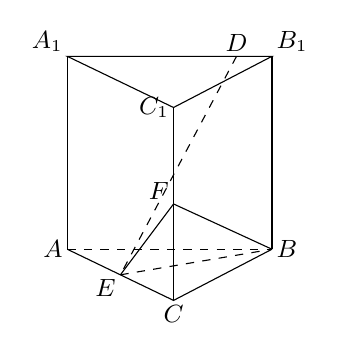
\begin{tikzpicture}[font=\small, line width=0.4pt,
  every node/.style={inner sep=1.5pt}]
  \coordinate (A1) at (0,3.00);   \coordinate (B1) at (2.60,3.00);
  \coordinate (C1) at (1.35,2.35);
  \coordinate (A)  at (0,0.55);   \coordinate (B)  at (2.60,0.55);
  \coordinate (C)  at (1.35,-0.10);
  \coordinate (D)  at (2.15,3.00);
  \coordinate (E)  at (0.675,0.225);
  \coordinate (F)  at (1.35,1.125);
  % 上底面
  \draw (A1) -- (B1) -- (C1) -- cycle;
  % 侧棱
  \draw (A1) -- (A);  \draw (B1) -- (B);  \draw (C1) -- (C);
  % 下底面：后棱 AB 被遮挡
  \draw[dashed] (A) -- (B);
  \draw (A) -- (C) -- (B);
  % 辅助线
  \draw (B) -- (F);          % BF
  \draw (E) -- (F);          % EF（三棱锥 F-EBC 的棱）
  \draw[dashed] (E) -- (B);  % EB（内部，被遮挡）
  \draw[dashed] (D) -- (E);  % DE
  % 顶点标注
  \node[anchor=south east] at (A1) {$A_1$};
  \node[anchor=south west] at (B1) {$B_1$};
  \node[anchor=south]      at (D)  {$D$};
  \node[anchor=east]       at (C1) {$C_1$};
  \node[anchor=east]       at (A)  {$A$};
  \node[anchor=west]       at (B)  {$B$};
  \node[anchor=north]      at (C)  {$C$};
  \node[anchor=north east] at (E)  {$E$};
  \node[anchor=south east] at (F)  {$F$};
\end{tikzpicture}
